\documentclass{article}
\usepackage{main}

\pagestyle{empty}
\title{Distance entre deux points}
\author{}
\date{26 Février 2024}


\begin{document}
\maketitle
\thispagestyle{empty}
\section{Corde à noeuds}
Une technique utilisée lors de l'Antiquité dans la construction était de se servir d'une \og corde à 13 noeuds \fg (bien que cet usage ne soit pas totalement attesté par les historiens). Il s'agit d'une corde séparée en $12$ sections égales. Pour s'assurer qu'un mur est droit, les bâtisseurs attachaient la corde au sol et formaient le triangle suivant en s'aidant du sol et du mur. La portion de corde contre le sol mesure $4$ sections de corde, celle contre le mur en mesure $3$. Il ne reste à vérifier que le dernier côté du triangle mesure bien $5$ sections de corde.
\begin{center}
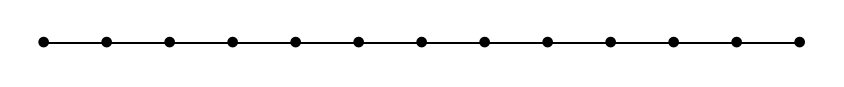
\begin{tikzpicture}[scale=0.8]
\foreach \i in {0,1,...,12} \draw (\i,0) node {$\bullet$};
\draw (0,0) -- (12,0);
\end{tikzpicture}
\vspace{0.5cm}
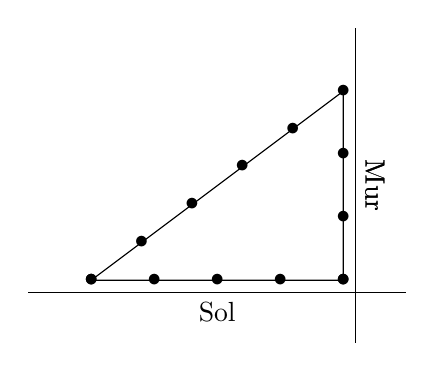
\begin{tikzpicture}[scale=0.8]
\coordinate (A) at (0,0);
\coordinate (B) at (4,0);
\coordinate (C) at (4,3);
\coordinate (MH) at (4.2,4);
\coordinate (MB) at (4.2,-1);
\coordinate (SG) at (-1,-0.2);
\coordinate (SD) at (5,-0.2);
\draw (A) -- (B) -- (C) -- cycle;
\draw (MH) -- (MB) node[midway,sloped,above] {Mur};
\draw (MH) -- (MB) node[midway,sloped,above] {Mur};
\draw (SG) -- (SD) node[midway,below] {Sol};
\foreach \i in {0,1,...,4} \draw (\i,0) node {$\bullet$};
\foreach \j in {0,1,...,3} \draw (4,\j) node {$\bullet$};
\foreach \x in {0,1,...,4} \draw (\x *4/5,3/5 * \x) node {$\bullet$};
\end{tikzpicture}
\end{center}
\paragraph{Question} Quel résultat mathématique permet de justifier que le mur est droit grâce à la corde à $13$ noeuds ?
\newpage
\section{Dans l'autre sens}
Grâce au théorème de Pythagore, nous pouvons donc montrer qu'un triangle est rectangle en mesurant ses côtés. Maintenant, nous allons faire l'inverse : nous allons mesurer un segment en faisant apparaître un triangle rectangle.
\subsection*{Premiers Pas}
Soit un repère orthonormé $(O;I;J)$.
\begin{center}
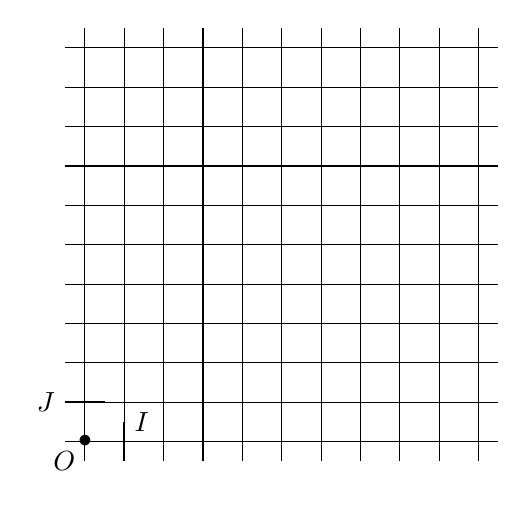
\begin{tikzpicture}
\draw (-0.25,-0.25) grid[step=0.5] (5.25,5.25);
\draw (0,0) node {$\bullet$} node[below left] {$O$};
\draw[thick] (0.25,0.5) -- (-0.25,0.5) node[left] {$J$};
\draw[thick] (0.5,-0.25) -- (0.5,0.25) node[right] {$I$};
\end{tikzpicture}
\end{center}
\paragraph{Questions}
\begin{enumerate}[label=\emph{\alph*)}]
\item Placer le point $A(4;0)$ sur le repère. Quelle est la distance $OA$ ?
\item Placer le point $B(0;3)$ sur le repère. Quelle est la distance $OB$ ?
\item Placer le point $C(4;3)$ sur le repère. Quelle est la nature du triangle $OAC$ ?
\item En utilisant les résultats décrits à la première section, en déduire la longueur $OC$.
\item Placer les points $D(5;5)$, $E(9;5)$ et $F(9;8)$. Quelle est la nature du triangle $DEF$ ? En déduire directement la longueur $DF$.
\end{enumerate}
\subsection*{Deuxieme exemple}
On pose $P(-2;3)$ et $Q(1;3)$. On cherche à calculer la longueur $PQ$. 
\paragraph{Question} 
Tracer un repère et y représenter $P$ et $Q$. Placer un point $R$ tel que :
\begin{itemize}
\item $PQR$ est un triangle rectangle en $R$;
\item Les distances $PR$ et $QR$ s'obtiennent immédiatement par lecture graphique.
\end{itemize}
En déduire la longueur $PQ$ à l'aide du théorème de Pythagore.
\end{document}